\documentclass[a4paper]{article}
\usepackage{ makeidx,amsmath, amsthm,amssymb,enumerate, graphicx,amsfonts, hyperref}
\newtheorem{mydef}{Definition}

\begin{document}
\begin{center}
{\bf{\huge CS 373 }}\\
{\bf{\huge a.k.a. Theory of Computation}}\\
\vspace{ 5 cm }
{\bf{\large Spring 2012, University of Illinos}}\\
{\bf{\large as taught by Steve LaValle }}\\
\vspace{ 1 cm }                         
{\large notes by Michele R. Esposito}\\
\vspace{ 5cm }
Please, let report any error or type-o at \underline{\href{mailto:micheleresposito@gmail.com}{ micheleresposito@gmail.com }}

\end{center}
\newpage
\tableofcontents
\newpage
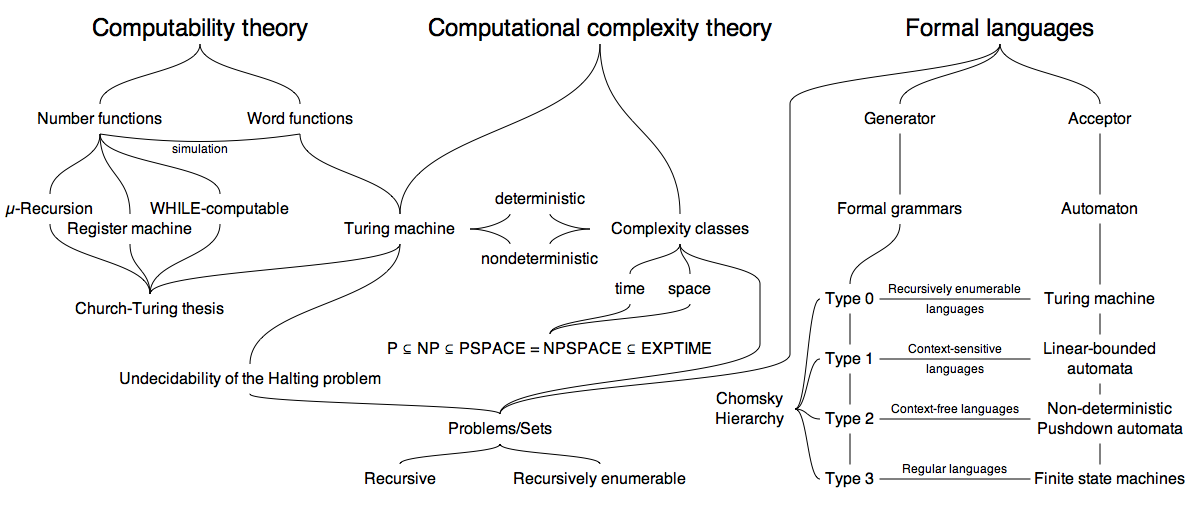
\includegraphics[scale=.38]{computer_theory.png}

% =========================================================

\section{Basic Definitions} % (fold)
\label{sec:Basic Definitions}
\subsection{String} % (fold)
\label{sub:String}
A {\bf string over an alphabet} is a finite sequence of symbols form that alphabets.
% subsection String (end)
\subsection{Language} % (fold)
\label{sub:Language}
A {\bf language} is a set of strings.
% subsection Language (end)
\subsection{Alphabet} % (fold)
\label{sub:Alphabet}
A finite set of object called symbols
% subsection Alphabet (end)
\subsection{Empty string} % (fold)
\label{sub:Empty string}
The string of length zero
% subsection Empty string (end)
% section Basic Definitions (end)

% =========================================================

\section{Regular Languages} % (fold)
\label{sec:Regular Laguages}
\index{Regular Languages}
\subsection{DFAs} % (fold)
\label{sub:Finite Automaton}
A {\bf finite automaton} is a 5-tuple $(Q,\Sigma,\delta,q_0,F)$ where,
\begin{enumerate}
  \item Q is a finite set called the {\bf states}
  \item $\Sigma$ is a finite set called the {\bf alphabet}.
  \item $\delta:Q \times \Sigma \rightarrow Q$ is the {\bf transition function}.
  \item $q_0 \in Q$ is the {\bf start state}
  \item $F \subseteq Q$ is the {\bf set of accept states}.
\end{enumerate}
We say that a machine $M$ accepts $w$ if a sequence of states $r0,r1,\dots,r_n \in Q$ exists with three conditions:
\begin{enumerate}
  \item $r_0=q_0$
  \item $\delta(r_i,w_{i+1})= r_{i+1}$, for $i=0,\dots,n-1$.
  \item $r_n \in F$.
\end{enumerate}
We say that M {\bf recognizes language} A if $A=\left\{ w | M \text{ accepts }w \right\}$.
% subsection Finite Automaton (end)

\subsection{Regular language} % (fold)
\label{sub:Regular language}
A language is called a {\bf regular language} if some finite automaton recognizes it.
% subsection Regular language (end)

\subsection{The regular operations} % (fold)
\label{sub:The regular operations}
Let A and B be languages. We define the regular operations {\bf union,concatenation,} and {\bf star} as follows:
\begin{itemize}
  \item {\bf Union} $A \cup B= \left\{ x|x \in A \text{ or } x \in B \right\}$. 
  \item {\bf Concatenation} $AB=\left\{ xy|x \in A \text{ and } y \in B \right\}$.
  \item {\bf Star}: $A^*=\left\{ x_1x_2\dots x_k| k \geq 0 \text{ and each }x_i \in A \right\}$. Otherwise, can be defined
    recursively as: $V_0={\epsilon}$, then $V_{i+1}=\{wv| w \in V_i \text{ and } v \in V\}$ where $i \geq0$. Then,
    $V^*=\bigcup_{i\in \mathbb{N}} V_i$. REMEMBER! $\varnothing^*=\left\{ \epsilon \right\}$
\end{itemize}
The set of regular languages is closed under the following operations: (taken from Wikipedia)
\begin{enumerate}
  \item Union: $K \cup L$.
  \item Intersection: $K \cup L$.
  \item Complement: $K^c$.
  \item Difference: $K-L$.
  \item Kleene star: $K^*$.
  \item String homomorphism, inverse homomorphism. See section 2.8 for details.
  \item Reverse: $K^R$.
  \item Quotient: $L_1 \backslash L_2$. See section 2.8 for details.
\end{enumerate}
% subsection The regular operations (end)
\subsection{NFAs} % (fold)
\label{sub:NFAs}
A {\bf NFA} is a 5-tuple $(Q,\Sigma, \delta, q_0, F)$, where

\begin{enumerate}
  \item Q is a finite set called the {\bf states}
  \item $\Sigma$ is a finite set called the {\bf alphabet}.
  \item $\delta:Q \times \Sigma_{\epsilon} \rightarrow 2^Q$ is the {\bf transition function}.
  \item $q_0 \in Q$ is the {\bf start state}
  \item $F \subseteq Q$ is the {\bf set of accept states}.
\end{enumerate}
$2^Q$ is the power set.
% subsection NFAs (end)
\subsection{Regular expression} % (fold)
\label{sub:Regular expression}
Say that R is a {\bf regular expression} if R is
\begin{enumerate}
  \item $a$ for some $a$ in the alphabet $\Sigma$.
  \item $\epsilon$.
  \item $\varnothing$
  \item $R_1 \cup R_2$ where $R_1$ and $R_2$ are regular expressions
  \item $R_1 R_2$ where $R_1$ and $R_2$ are regular expressions
  \item $R_1^*$ where $R_1$ is a regular expression.
\end{enumerate}
% subsection Regular expression (end)
\subsection{GNFAs} % (fold)
\label{sub:GNFAs}
A {\bf generalized nondeterministic finite automaton } is 5-tuple $(Q,\Sigma, \delta, q_{start}, q_{accept})$, where

\begin{enumerate}
  \item Q is a finite set called the {\bf states}
  \item $\Sigma$ is a finite set called the {\bf alphabet}.
  \item $\delta:Q \times \Sigma_{\epsilon} \rightarrow R$ is the {\bf transition function}.
  \item $q_0 \in Q$ is the {\bf start state}
  \item $F \subseteq Q$ is the {\bf set of accept states}.
\end{enumerate}
% subsection GNFAs (end)
\subsection{Pumping lemma} % (fold)
\label{sub:Pumping lemma}
if $A$ is a regular language, then there is a number $p$ (the pumping length) where, if $s$ is any string in $A$ of length
at least $p$, then $s$ may be divided into three pieces, $s=xyz$, satisfying the conditions:
\begin{enumerate}
  \item for each $i\geq 0$, $xy^iz \in A$,
  \item $|y| > 0$, and
  \item $|xy| \leq p$.
\end{enumerate}
Imagine there is an ``adversary''. He gets to pick: $p$, breaks $s$ into $xyz$. You get to pick $s$ and $i$. Use to prove irregularity by contradiction.
% subsection Pumping lemma (end)
% section Regular Laguages (end)
% =========================================================
\subsection{Closure Proprieties of Regular Sets} % (fold)
\label{sub:Substitution and homomorphism}
{\bf Substitution} \\
The class of regular sets has the interesting propriety that it is closed under substitution. $\forall a \in \Sigma$ of a regular
subset $R$, let $R_a$ be a particular regular set. Suppose that we replace each word $a_1a_2\dots a_n \in R$ by the set of words of the form $w_1w_2 \dots w_n$, where $w_i$ is an $substitution$ mapping of an alphabet $\Sigma$ onto subset of $\Delta^*$.
The mapping $f$ is extended to the strings as follows: \\
\begin{enumerate}
  \item $f(\epsilon)=\epsilon$;
  \item $f(xa)=f(x)f(a)$.
\end{enumerate}
The mapping $f$ is extended to the languages by defining $f(L)=\bigcup_{x \in L}f(x)$. \\
{\bf Homomorphism} \\
A homomorphism $h$ is a substitution s.t. $h(a)$ contains a single string for each $a$. We generally take $h(a)$ to be the string itself, rather than the set containing that string. \\
{\bf Inverse homomorphism} \\
An $inverse$ $homomorphism$ of a language $L$ be:
\begin{center}
  $h^{-1}(L)=\left\{ x|h(x) \in L \right\}$
\end{center}
Or, using a string:
\begin{center}
  $h^{-1}(w)=\left\{ x|h(x) = w \right\}$
\end{center}
{\bf Quotients of languages} \\
Define the $quotient$ of languages $L_1$, $L_2$, written $L_1,L_2$ to be:
\begin{center}
  $\left\{ x| \exists y \in L_2 \text{ such that } xy \in L_1 \right\}$.
\end{center}
% subsection Substitution and homomorphism (end)
\subsection{Myhill-Nerode Theorem} % (fold)
\label{sub:Myhill-Nerode Theorem}
{\bf Right invariant} \\
An equivalence relation $R$ s.t. $xRy$ implies $xzRyz$ is said to be $right$ $invariant$. We see that every finite automaton induces a right invariant equivalence relation, on its set of input strings. \\
{\bf Myhill-Nerode Theorem} \\
The following three statements are equivalent:
\begin{enumerate}
  \item The set $L \subseteq \Sigma^*$ is accepted by some finite automaton.
  \item $L$ is the union of some of the equivalence classes of a right invariant equivalence relation of finite index.
  \item Let equivalence relation $R_l$ be defined by: $xR_Ly$ if and only if $\forall z \in \Sigma^*$, $xz$ is in 
    $L$ exactly when $yz$ is in $L$. Then $R_L$ is of finite index.
\end{enumerate}
We can use the Myhill-Nerode theorem to prove nonregularity. For a language A over $\Sigma$, the relation $~A$ has a finite number of equivalence classes iff $A$ is regular. This, we can prove nonregularity by:
\begin{enumerate}
  \item Choose some infinite set $S \subseteq \Sigma^*$;
  \item Show that $x,y \in S, x \neq y$ belongs to different equivalence classes. Thus, $\exists z$ s.t. $ xz \in A$, but 
    $yz \notin A$.
  \item Since $S$ is infinite and every member has a ≠ equivalence class, $~A$, does not have a finite index. By the Myhill-Nerode theorem, $A$ is nonregular. (condition 3).
\end{enumerate}
% subsection Myhill-Nerode Theorem (end)
\section{Context-Sensitive Languages} % (fold)
\label{sec:Context-Free Languages}
\subsection{Context-free grammars} % (fold)
\label{sub:Context-free grammars}
A {\bf context-free grammar} is a 4-tuple $(V,\Sigma,R,S)$, where
\begin{enumerate}
  \item $V$ is a finite set called the $variables$, or $nonterminals$,
  \item $\Sigma$ is a finite set, disjoint from V, called the {\bf terminals},
  \item $R$ is a finite set of {\bf rules}, with each rule being a variable and string of variables and terminals, and
  \item $S \in V$ is the start variable.
\end{enumerate}
If $u,v$ and $w$ are strings of variables and terminals, and $A \rightarrow w$ is a rule of the grammar, we say that $uAv$ 
{\bf yields} $uwv$, written $uAv \implies uwv$. Say that $u$ {\bf derives} $v$, written $u \implies v$, if $u=v$ or if a sequence
$u_1,u_2,\dots,u_k$ exists for $k \geq 0$ and 
\begin{center}
  $u \implies u_1 \implies u_2 \implies \dots \implies u_k \implies v$
\end{center}
The {\bf language of the grammar} is $\left\{ w \in \Sigma^* | S \implies^* w \right\}$. \\

{\bf Ambiguity} \\
A string $w$ is derived {\bf ambiguously} in context-free grammar $G$ is it has two or more different leftmost
derivations. Grammar $G$ is {\bf ambiguous} if it generates some string ambiguously.

{\bf Chomsky Normal Form} \\
Chomsky normal form is useful in giving algorithms for working with context-free grammars. Also, is good for parsing, because it 
produces a binary tree. \\
A context-free grammar is in {\bf Chomsky normal form} if every rule is of the form \\
\begin{center}
  $ A \rightarrow BC$ \\
  $ A \rightarrow a$ \\
\end{center}
where $a$ is any terminal, and $A,B, \text{ and } C$ are any variables- except that $B$ and $C$ may not be the start variable.
In addition we permit the rule $S \rightarrow \epsilon$, where $S$ is the start variable. \\
Any context-free language is generated by a context-free grammar in Chomsky normal form.
% subsection Context-free grammars (end)

\subsection{Pushdown Automata} % (fold)
\label{sub:Push Down Automatas}
A pushdown automata is a type of NFA, but they have an extra component called stack, which allows them to have infinite memory.
They have the same power as context-free grammar, as we will see later. Here is a schematic representation of a PDA. \\
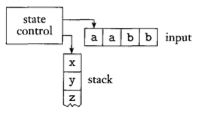
\includegraphics[scale=.6]{pda-scheme.png} \\
Now, here is a formal definition of a PDA. A {\bf pushdown automaton} is a 6-tuple $\left( Q,\Sigma, \Gamma, \delta, q_0, F \right)$ where $Q,\Sigma,\Gamma$ and $F$ are all finite sets, and
\begin{enumerate}
  \item $Q$ is the set of states,
  \item $\Sigma$ is the input alphabet,
  \item $\Gamma$ is the stack alphabet,
  \item $\delta: Q \times \Sigma_\epsilon \times \Gamma_\epsilon \rightarrow 2^{Q \times \Gamma_\epsilon}$ is the transition function,
  \item $q_o \in Q$ is the start state, and
  \item $F \subseteq Q$ is the set of accept states.
\end{enumerate}
A pushdown automaton $M=(Q,\Sigma,\Gamma,\delta,q_o,F)$ computes as follows, It accepts input $w$ if $w$ can be written as $w=w_1w_2\dots w_m$, where each $w_i \in \Sigma_\epsilon$ and sequences of states $r_0,r_1,\dots , r_m \in Q$ and string $s_0, s_1, \dots
, s_m \in \Gamma^*$ exist that satisfy the following three conditions. The string $s_i$ represents the sequence of stack contents
that $M$ has on the accepting branch of the computation.
\begin{enumerate}
  \item $r_0 = q_0$ and $s_0 = \epsilon$. This condition signifies that $M$ starts out properly, in the start state and with an
    empty stack.
  \item For $i=0, \dots, m-1$, have $(r_{i+1}, b) \in \delta(r_i,w_{i+1},a)$, where $s_i = at$ and $s_{i+1}=bt$ for some
    $a,b \in \Gamma_\epsilon$ and $t \in \Gamma^*$. This condition states that $M$ moves properly according to the state, stack,
    and next input symbol.
  \item $r_m \in F$. This condition states that an accept state occurs at the input end.
\end{enumerate}
% subsection Push Down Automatas (end)

\subsection{Pumping Lemma for CFL} % (fold)
\label{sub:Pumping Lemma for CFL}
If $A$ is a context-free language, then there is a number $p$ where, if $s$ is any string in $A$ of the length at least $p$, then $s$ may be divided into five pieces $s=uvxyz$ satisfying the conditions:
\begin{enumerate}
  \item for each $i \geq 0, uv^ixy^iz \in A$,
  \item $|vy| > 0$, and 
  \item $|vxy| \leq p$.
\end{enumerate}
% subsection Pumping Lemma for CFL (end)

\subsection{Closure Properties of CFL's} % (fold)
\label{sub:Closure Properties of CFL's}
Context free languages are closed under the following operations:
\begin{enumerate}
  \item Union
  \item Concatenation
  \item Kleene star
  \item Substitution
  \item Homomorphism, and inverse homomorphism
  \item Reverse.
\end{enumerate}
% subsection Closure Properties of CFL's (end)
\subsection{Context-Sensitive grammars} % (fold)
\label{sub:Context-Sensitive grammars}
A {\bf context-sensitive grammar} is a formal grammar in which the left-hand sides and right-hand sides of any production rules may be surrounded by a context of terminal and nonterminal symbols. 
\begin{enumerate}
  \item V is a finite set of variables 
  \item $\Sigma$ is finite set of terminals, and $\Sigma \cap V = \varnothing$.
  \item R is a finite set of \underline{rules} of the form $\alpha A\beta\rightarrow\alpha \gamma\beta$ in which $A$ is a variable and $\alpha,\beta,\gamma$ are strings of terminals and variables.
  \item $S\in V$ is the start variable.
\end{enumerate}
% subsection Context-Sensitive grammars (end)
\subsection{CYK Algorithm} % (fold)
\label{sub:CYK Algorithm}
In order to test for membership of a certain string to a language, we can use the CYK algorithm. In order to do so, we first need to write the grammar in CNF. Then, given $x$ of length $n \geq 1$ and a grammar $G$, determine for each $i$ and $j$ and for each variable $A$, whether $A\implies^* x_{ij}$, where $xij$ is the substring of $x$ of length $j$ beginning at position $i$. To state the CYK.
% subsection CYK Algorithm (end)
% section Context-Free Languages (end)
\section{Turing Machines} % (fold)
\label{sec:Turing Machines}
A Turing machine is a 7-tuple $(Q,\Sigma,\Gamma,\delta,q_0,q_{accept},q_{reject})$ with $Q,\Sigma,\Gamma$ finite, nonempty sets.
\begin{enumerate}
 \item $Q$ is a set of states
  \item $\Sigma$ is the input alphabet, which does not contains the blank symbol.
  \item $\Gamma$ is the \underline{tape alphabet}, in which $blak \in \Gamma$, and $\Sigma \subset \Gamma$.
  \item $\delta: Q \times \Gamma \rightarrow Q \times\Gamma\left\{ L,R \right\} $ is the \underline{transition function}.
  \item $q_0 \in Q$ is the \underline{start state}.
  \item $q_{accept} \in Q$ is the \underline{accept state}
  \item $q_{reject} \in Q$ is the \underline{reject state}, and $q_{accept} \neq q_{reject}$.
\end{enumerate}
A Turing machine $M$ {\bf accepts } input $w$ if a sequence of configurations $C_1,C_2,\dotsc_k$ exists where
\begin{enumerate}
  \item $C_1$ is the start configuration of $M$ of input $w$,
  \item each $C_i$ yields $C_{i+1},$ and 
  \item $C_k$ is an accepting configuration.
\end{enumerate}
The collection of strings that $M$ accepts if the {\bf language of M}, denoted $L(M)$. \\
Call a language {\bf Turing-recognizable} if some Turing machine recognizes it. That is, the machine ends on accept states, or keeps looping. Therefore, a $TM$ recognizes $A$ if
\begin{itemize}
  \item Accepts it $x \in A$
  \item Loops it $x \notin A$
\end{itemize}
Call a language {\bf Turing-decidable} if some Turing machine decides it. That is, the machine always ends in an accept state. Therefore, a $TM$ decides $A$ if
\begin{itemize}
  \item Accepts if $x \in A$
  \item Rejects if $x \notin A$
\end{itemize}
% section Turing Machines (end)
\subsection{Variants of Turing machines} % (fold)
\label{sub:Variants of TUring machines}
There are some alternatives version of Turing machines. We call those {\bf variants} of Turing machine, and we analyze the power. For more details. In more detail, we look at two variants:
\subsubsection{Multitape Turing machine}
A {\bf multitape TM} is an ordinary TM with several tapes. WE define the transition function to be
\begin{align}
  \delta:Q\times\Gamma^k\rightarrow Q\times\Gamma^k\times\left\{ L,R,S \right\}^k
\end{align}
Where $k$ is the number of tapes. the expression $\delta(q_1,a_1,\dots,a_k)=\left( q_j,b_1,\dots,b_k,L,R,\dots,L \right)$ means that if the machine is in state $q_i$ and heads 1 through $k$ are reading symbols $a_1$ through $a_k$, then machine goes to state $q_j$, writes symbols $b_1$ through $b_k$, and directs each head with proper movement. \\
\underline{Theorem:} Every multitape Turing machine has an equivalent single-tape Turing machine. Look at lecture notes for proof detail.
\subsubsection{Nondeterministic Turing Machines}
A NTM is a TM which at any point in computation can move in several possible ways. The transition function has the form
\begin{align}
  \delta:Q\times\Gamma\rightarrow2^{Q\times\Gamma\times\left\{ L,R \right\}}
\end{align}
The computation of a NTM is a tree whose branches correspond to $\neq$ possibilities for the machine. If some branch of the computation leads to the accept state, the machine accepts its input. \\
\underline{Theorem:} Every Nondeterministic Turing machine has an equivalent deterministic TM. Look at lecture notes for proof detail. 
% subsection Variants of TUring machines (end)
\subsubsection{Enumerators}
An \underline{enumerator} is a TM with an ``attached printer'', which is used to output strings. An enumerator E starts with a blank input tape. If the enumerator doesn't halt, it may print infinite strings. The language enumerated by E is a collection of all the strings that it eventually prints out. Moreover, E may generate the strings of the language in a ny order, possibly with repetitions. \\
\underline{Theorem:} A language is Turing-recognizable iff some  enumerator enumerates it.

\subsection{Definition of algorithms} % (fold)
\label{sub:Definition of algorithms}
The {\bf Church-Turing} thesis provides a definition of an algorithm. That is, the intuitive notion of algorithms equals Turing machine algorithms.
% subsection Definition of algorithms (end)
\section{Decidability} % (fold)
\label{sec:Decidibility}
We now begin to investigate the power of algorithms. In fact, in this section we will look at which problems are solvable by using the power of algorithms.
\subsection{Decidable languages} % (fold)
\label{sub:Decidable languages}
The following languages, and machines, can be simulated into a universal Turing machine. Here are the machines, with a descriptions of the algorithms.
\begin{enumerate}[{\bf (a)}]
  \item ${\bf A_{DFA}}=\left\{ <B,w> | B \text{ if a DFA that accepts input string }w \right\}$. Then, $A_{DFA}$ is decidable with the following algorithm:\\
    $M=$``on input$<B,W>$, where $B$ is a DFA and $w$ is a string:
      \begin{enumerate}[1.]
        \item Simulate $B$ on input $w$.
        \item if the simulation ends in an accept state, \emph{accept}, If it ends in a non accepting state, \emph{reject}.
      \end{enumerate}

    \item An  ${\bf A_{NFA}}=\left\{ <B,w>| B \text{ is an NFA that accepts input string }w \right\}$ is a decidable language. Here is a turing machine $M$ that accepts it:\\
      $N=$``On input $<B,w>$ where $B$ is an $NFA$, and $w$ is a string:
      \begin{enumerate}[1.]
        \item Convert NFA $B$ to an equivalent $DFA C$. 
        \item Simulate $B$ on input $w$.
        \item if the simulation ends in an accept state, \emph{accept}, If it ends in a non accepting state, \emph{reject}.
      \end{enumerate}

    \item ${\bf A_{REX}}=\left\{ <R,w>| \text{ R is a regular expression that generates string }w \right\}$.\\
      $P=$`` On input $<R,w>$ where $R$ is a regular expression and $w$ is a string:
      \begin{enumerate} [1.]
        \item Convert regular expression $R$ to an equivalent DFA A by using the procedure for for this conversion.
        \item Simulate $B$ on input $w$.
        \item if the simulation ends in an accept state, \emph{accept}, If it ends in a non accepting state, \emph{reject}.
      \end{enumerate}

    \item  ${\bf E_{DFA}}= \left\{ <A> | A \text{ is a DFA and }L(A)=\varnothing \right\}$ is a decidable language\\ 
      $T=$``On input $<A>$ where $A$ is a $DFA$:
      \begin{enumerate}[1.]
        \item Mark the start state of A.
        \item Repeat until no new states get marked:
        \item Mark any state that has a transition coming into it from any state that is already marked
        \item If no accept state is marked, \emph{accept}; otherwise \emph{reject}.''
      \end{enumerate}

    \item ${\bf A_{CFG}}=\left\{ <G,w>|G \text{ is a CFG that generates string} w \right\}$. Define the TM $S$ for $A_{CFG}$ as follow: \\
      $S=$``On input $<G,w>$, where $G$ is a $CFG$ and $w$ is a string:
      \begin{enumerate}[1.]
        \item Convert $G$ to an equivalent grammar in Chomsky normal form
        \item List all derivations with $2n-1$ steps, where $n=|w|$. If $n=0$, then list all derivations with 1 step.
        \item If any of these derivations generate $w$, \emph{accept}; if not \emph{reject}.''
      \end{enumerate}

    \item  ${\bf E_{CFG}}= \left\{ <A> | A \text{ is a CFG and }L(A)=\varnothing \right\}$ is a decidable language. \\
    \item Every context-free language is decidable.
\end{enumerate}
\subsection{The Halting problem} % (fold)
\label{sub:The Halting problem}
Let $A_{TM}=\left\{ <M,w> | M \text{ is a TM and M accepts }w \right\}$. Then, $A_{TM}$ is undecidable. This proof, which is in the lecture notes, is based on construction a decider $H$ and $D$ that, when they run on the description of themselves, they will lead to a contradiction. This is a rough sketch of the machine, and of the proof:\\
Let $H$ be a decider such that
\begin{align}
  H(<M,w>)=
  \begin{cases}
    accept \hspace{.5 cm} \text{ if M accepts} w \\
    reject \hspace{.5 cm} \text{ if M does not} w \\
  \end{cases}
\end{align}
Now, construct $D$, having $H$ as a subroutine: \\
$D="$On input <M>, where $M$ is a TM:
\begin{enumerate}
  \item Run H on input $<M,<M>>$.
  \item Output the opposite of what $H$ outputs.
\end{enumerate}
Therefore, we have the following steps:
\begin{itemize}
  \item $H$ accepts $<M,w>$ exactly when $M$ accepts $w$.
  \item $D$ rejects $<M>$ exactly when $M$ accepts $<M>$.
  \item $D$ rejects $<D>$ exactly when $D$ accepts $<D>$.
\end{itemize}
Note that the final step obviously leads to a contradiction, therefore the machines $H$ and $D$ cannot exists.
% subsection The Halting problem (end)
\subsection{A Turing unrecognizable language} % (fold)
\label{sub:A turing unrecognizable language}
Recall that the complement of a language is the language consisting of all strings that re not in the language. We say that a language is {\bf co-Turing-recognizable} if it the complement of a Turing-recognizable language.\\
\underline{Theorem:} A language is decidable iff it is Turing-recognizable and co-Turing-recognizable. \\
That is, a language is decidable exactly when both it and its complement are Turing-recognizable.
\underline{Corollary:} $\bar{A_{TM}}$ is not Turing-recognizable. \\
{\bf Proof:} We know that $A_{TM}$ is Turing-recognizable. If $\bar{A_{TM}}$ also were Turing-recognizable, $A_{TM}$ would be decidable. Theorem 4.11 tells us that $A_{TM}$ is not decidable, so $\bar{A_{TM}}$ must not be Turing-recognizable
% subsection A turing unrecognizable language (end)
% subsection Decidable languages (end)
% section Decidability (end)
\section{Reducibility} % (fold)
\label{sec:Reductibility}
A {\bf reduction} is a ways of converting one problem into another problem in such a way that a solution to the second problem can be used to solve the first problem. Reducibility plays an important role in classifying problems by decidability and later in complexity theory as well. 
\subsection{Undecidable problems from language theory} % (fold)
\label{sub:Undecidable problems from language theory}
Let's try to establish the undecidability of few problems. Let $HALT_{TM}$ be:
\begin{align}
  HALT_{TM} = \left\{ <M,w>| \text{ M is a TM and M halt on input }w \right\}.
\end{align}
Then, we can establish that $HALT_{TM}$ is undecidable, with the following proof:
Let's assume for the purposes of obtaining a contradiction that $TM$ $R$ decides $HALT_{TM}$. We construct $TM S$ to decide $A_{TM}$, with $S$ operating as follows. \\
$S="$On input $<M,w>$, and encoding of a $TM M$ and a string $w$:
\begin{enumerate}[{\bf 1.}]
  \item Run TM R on input $<M,w>$.
  \item If R rejects, \underline{reject}.
  \item If R accepts, simulate $M$ on $w$ until it halts.
  \item If $M$ has accepted, \underline{accept}; if $M$ has rejected, \underline{reject}.``
\end{enumerate}
Clearly, if $R$ decides $HALT_{TM}$, then $S$ decides $A_{TM}$. Then, $HALT_{TM}$ must be undecidable. \\

{\bf The following languages are all undecidable:}
\begin{itemize}
    %E_TM
    \item ${\bf E_{TM}}=\left\{ <M>| \text{M is a TM and L(M)}=\varnothing \right\}$. Here is the proof. \\
   First, construct a machine $M_1$ so that: \\
   $M_1=$``On input $x$:
   \begin{enumerate}
     \item if $x\neq w$, \underline{reject}
     \item if $x=w$, run $M$ on input $w$ and \underline{accept} if M does''.
   \end{enumerate}
   Now, assume that TM $R$ decides $E_{TM}$ and construct TM $S$ that decides $A_{TM}$ as follows: \\
   $S=$``On input $<M,w>$, and encoding of a TM $M$ and a string $w$:
   \begin{enumerate}
     \item Use the description of $M$ and $w$ and construct the TM $M_1$ just described
     \item Run $R$ on input $<M_1>$
     \item If $R$ accepts, \underline{reject}; if $R$ reject, \underline{accept}.
   \end{enumerate}
  %REGULAR_TM
  \item ${\bf REGULAR_{TM} }=\left\{ <M>|M \text{ is a TM and L(M) is regular language} \right\}$ is undecidable. \\

    {\bf Proof idea:} We assume that $REGULAR_{TM}$ is decidable by a TM $R$ and use this assumption to construct a TM $S$ that decides $A_{TM}$. The idea is for $S$ to take its input $<M,w>$ and modify $M$ so that the resulting TM recognizes a regular language iff M accepts $w$. We call the modified machine $M_2$. We design $M_2$ to recognize the nonregular language $\left\{ 0^n1^n|n\geq0 \right\}$ if $M$ does not accept $w$. \\
    {\bf Proof:} We let $R$ be a TM that decides $REGULAR_{TM}$ and construct TM $S$ to decide $A_{TM}$. Then $S$ works in the following manner: \\
    $S="$On input $<M,w>$, where $M$ is a TM and $w$ is a string:\\
    \begin{enumerate}[{\bf 1.}]
      \item Construct the following TM $M_2$. \\
        $M_2=$'On input $x$: \\
        \begin{enumerate}
          \item If $x$ has the form $0^n1^n$, \emph{accept}.
          \item If $x$ does not have this form, run $M$ on input $w$ and accept if $M$ accepts $w$.'
        \end{enumerate}
      \item Run $R$ on input $<M_2>$.
      \item If $R$ accepts, \emph{accept}; if $R$ rejects, \emph{reject}.''
    \end{enumerate}
   %EQ_TM
   \item ${\bf EQ_{TM}} =\left\{ <M_1,M_2>|M_1 \text{ and }M_2 \text{ are TMs and} 
     L(M_1)=L(M_2)\right\}$ is undecidable \\
    {\bf Proof Idea: }Show that if $EQ_{TM}$ were decidable, $E_{TM}$ also would be decidable, by giving a reduction from $E_{TM}$ to $EQ_{TM}$. If one of these languages happens to be $\varnothing$, we end up with the problem of determining whether the language of the other machine is empty- that is, the $E_{TM}$ problem. So in a sense, the $E_{TM}$ problem is a special case of the $EQ_{TM}$ \\
    {\bf Proof:} We let TM $R$ decide $EQ_{TM}$ and construct TM $S$ to decide $E_{TM}$ as follows. \\
    $S=$``On input $<M>$, where $M$ is a TM: \\
    \begin{enumerate}[{\bf 1.}]
      \item Run $R$ on input $<M,M_1>$, where $M_1$ is a TM that rejects all inputs.
      \item If $R$ accepts, \emph{accept}; if R rejects, \emph{reject}.''
    \end{enumerate}
    If $R$ decides $EQ_{TM}$, $S$ decides $E_{TM}$, which is a contradiction.
\end{itemize}
% subsection Undecidable problems from language theory (end)
\subsection{Mapping reducibility} % (fold)
\label{sub:Mapping reducibility}
The intent of this section is that of formalizing reducibility. Doing so allows us to use reducibility in more refined ways, such as for proving that certain languages are not Turing-recognizable and for applications is complexity theory.\\
Being able to reduce problem A to problem B by using a mapping reducibility means that a computable function exists that converts instances of problem $A$ to instances of problem $B$. If we have such a conversion function, called a \emph{reduction}, we can solve by first using the reduction to convert it to an instance of $B$ and then applying to the solver for $B$.\\
\subsubsection{Computable functions}
A Turing machine computes a function by starting with the input to the function on the tape and halting with the output of the function on the tape.\\
\underline{Definition:} a function $f:\Sigma^*\rightarrow\Sigma^*$ is a {\bf computable function} if some Turing machine $M$, on every input $w$, halts with just $f(w)$ on its tape.
\subsubsection{Formal definition of mapping reducibility}
Language $A$ is {\bf mapping reducible} to a language $B$, written $A \leq_m B$, if there is a computable function $f:\Sigma^*\rightarrow\Sigma^*$, where for every $w$,
\begin{align}
  w\in A \leftrightarrow f(w)\in B
\end{align}
The function $f$ is called the {\bf reduction} of $A$ to $B$.\\
The test whether $w\in A$, we use the reduction $f$ to map $w$ to $f(w)$ and test whether $f(w)\in B$. The term \emph{mapping reduction} comes from the function or mapping that provides the means of doing the reduction.\\
\underline{Theorem:} \\
If $A \leq_m B$ and $B$ is decidable, then $A$ is decidable.\\
Also, its contrapositive works: \\
If $A\leq_mB$ and $A$ is undecidable, then $B$ is undecidable.
We can computer the reduction $A_{TM} \leq_M HALT_{TM}$ with the following TM $F$ that computers a reduction $f$:\\
$F=$``On input $<M,w>$:
\begin{enumerate}[{\bf 1.}]
  \item Construct the following machine M'. \\
    $M'=$''On input $x$:
    \begin{enumerate}
      \item Run $M$ on $x$.
      \item If $M$ accepts, \emph{accept}.
      \item If $M$ rejects, enter a loop.'
    \end{enumerate}
  \item Output $<M',w>$.``
\end{enumerate}
So, if a language is in $A$, then it will also be in $HALT$, because we accept. However, if the language is not in $A$, then we reject, and we keep halting in $HALT$.

% subsection Mapping reducibility (end)
\subsection{Rice's theorem} % (fold)
\label{sub:Rice's theorem}
{\bf Rice's Theorem} states that, for any non-trivial property of partial functions, there is no general and effective method to decide whether an algorithm computes a partial function with that property. Formally states:
Let $P$ be any property about TMs that so
\begin{enumerate}
  \item For every TMs $M_1$ and $M_2$, such that $L(M_1)=L(M_2)$, $<M_1>\in P$ iff $<M_2> \in P$
  \item There exists TMs $M_1$ and $M_2$ for which $<M_1>\in P$ and $<M_2> \notin P$.
\end{enumerate}
Trivial means that every TM has that property. For example, the language of a Turing machine has characters is trivial. \\
That is, a Turing machine cannot decide whether another Turing machine has that property. We have $L(M_1)=L(M_2)$ because we care about every Turing machine that has that language, regardless of its implementation.
% subsection Rice's theorem (end)
% section Reducibility (end)
\section{Complexity Theory} % (fold)
\label{sec:Complexity Theory}
Even if a problem is decidable, we want to be able to analyze the time and space that are required to solve that problem. Our objective in this chapter is to present the basic time requirements to solve such a problem. 
\subsection{Measuring complexity} % (fold)
\label{sub:Measuring complexity}
We \underline{analyze} the algorithms to determine how much time it uses. The number of steps that an algorithm uses on a particular input may depend on several parameters. For instance, if the input is a graph, the number of steps may depend on the number of steps may depend on the number of nodes. We compute the running time of an algorithm purely as a function of length of the string representing the input and don't consider any other parameters. In {\bf worst-case analysis}, we consider the longest possible running time. In {\bf average-case analysis}, we consider the average of all the running times of inputs of a particular length. \\
\subsubsection{Running time}
Let $M$ be a deterministic TM that halts on all inputs. The {\bf running time} or {\bf time complexity} of M is the function $f:\mathbb{N}\rightarrow\mathbb{N}$, where $f(n)$ is the maximum number of steps that $M$ uses on any input of length $n$. If $f(n)$ is the running time of $M$, we say that $M$ runs in time $f(n)$ and that $M$ is an $f(n)$ time TM. Customarily we use $n$ to represent the length of the input. 
% subsection Measuring complexity (end)
\subsection{Big-O and Small-O Notation} % (fold)
\label{sub:Big-o and small-O Notatio}
Because the exact running time of an algorithm often is a complex expression, we analyze the {\bf asymptotic analysis}. We do so by considering only the highest order term of the expression for the running time of the algorithm, disregarding both the coefficient of that term and any lower ordure terms.
\subsubsection{Big O:}
Let $f$ and $g$ be functions, $f,g:\mathbb{N}\rightarrow\mathbb{R}^+$. Say that $f(n)=O(g(n))$ if positive integers $c$ and $n_0$ exist such that $\forall n\geq n_0$
\begin{align}
  f(n)\leq cg(n)
\end{align}
Then, $g(n)$ is an {\bf upper bound} for $f(n)$.
\subsubsection{Small-o notation}
Frequently we derive bounds of the form $n^c$ for $c\geq0$. Such bounds are called {\bf polynomial bounds}. Bounds of the form $2^{n^\theta}$ are called {\bf exponential bounds} when $\theta\in\mathbb{R}, \theta>0$. To say that one function is asymptotically less than another, we use small -o notation:\\
Let $f$ and $g$ be function $f,g:\mathbb{N}\rightarrow\mathbb{R}^+$. Say that $f(n)=o(g(n))$ if
\begin{align}
  \lim_{n\rightarrow\infty}\frac{f(n)}{g(n)}=0
\end{align}
% subsection Big-o and small-O Notatio (end)
\subsection{Analyzing algorithms} % (fold)
\label{sub:Analyzing algorithms}
To analyze any algorithm, we consider each step in four separate stages. Then, we look at how they are linked and the collective result. we now set up some notation for classifying languages according to their time requirements: \\
Let $f:\mathbb{N}\rightarrow\mathbb{R}^+$ be a function. Define the {\bf time complexity class, TIME(t(n))}, to be the collection of all languages that are decidable by an $O(t(n))$ time TM.\\
% subsection Analyzing algorithms (end)
\subsection{Complexity relationship among models} % (fold)
\label{sub:Complexity relationship among models}
{\bf Theorem:} Let $t(n)$ be a function, where $t(n)\geq n$. Then every $t(n)$ time multitape Turing machine has an equivalent $O(t^2(n))$ time single-tape Turing machine.\\
{\bf Definition:} Let $N$ be a nondeterministic Turing machine that is a decider. Then {\bf running time} of $N$ is the function $f:\mathbb{N}\rightarrow\mathbb{N}$, where $f(n)$ is the maximum number  of steps that $N$ uses on any branch of its computation on any input of length $n$. \\
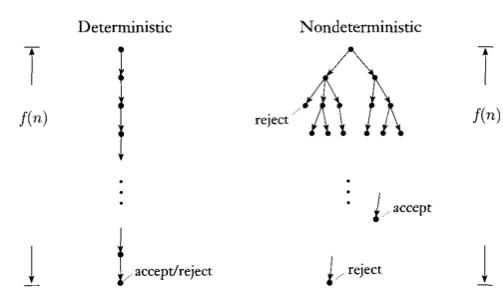
\includegraphics[scale=.5]{runtime.png}\\
{\bf Theorem:} Let $t(n)$ be a function, where $t(n)\geq n$. Then every $t(n)$ time nondeterministic single-tape TM has an equivalent $2^{O(t(n))}$ time deterministic single-tape TM.\\
% subsection Complexity relationship among models (end)
\subsection{The class P} % (fold)
\label{sub:The class P}
We consider polynomial differences in running time to be small, whereas exponential differences are considered to be large. The reason is that exponential time algorithms grow too fast to be useful for any practical purpose. They typically arise when we solve problems by using \underline{brute force search}. For example, one way to factor a number into its constituent primes is to search through all potential divisors.\\
\underline{Definition:} {\bf P} is the class of languages that are decidable in polynomial time on a deterministic single-tape Turing machine. In other words,
\begin{align}
  P=\bigcup_k TIME(n^k)
\end{align}
The class P is central in our theory because
\begin{enumerate}
  \item P is invariant $\forall$ models of computation that are polynomially equivalent to the deterministic single-tape Turing machine, and
  \item P roughly corresponds to the class of problems that are realistically solvable on a computer 
\end{enumerate}
\subsubsection{Examples of problems in P:}
\begin{itemize}
  \item PATH=$\left\{ <G,s,t>| G \text{ is a directed graph that has a directed path from }s \text{ to } t \right\}$
  \item RELPRIME=$\left\{ <x,y>|x \text{ and } y \text{ are relatively prime} \right\}$
  \item Every context-free language is a member of $P$.
\end{itemize}
% subsection The class P (end)
\subsection{The class NP} % (fold)
\label{sub:The class NP}
The problem of finding a {\bf Hamiltonian path} is said to be undecidable. That is,
HAMPATH: $\left\{ <G,s,t>|G \text{ is a directed graph with a Hamiltonian path from } s \text{ to }t \right\}$. This problem also has a feature called {\bf polynomial verifiability} that is important for understanding of complexity. Even though we don't know of a fast way to determine whether a graph contains a Hamiltonian path, if such a path were discovered somehow, we could easily convince someone else of its existence, by presenting it.\\
\begin{mydef}
  A {\bf verifier} for a language $A$ is an algorithm $V$, where
  \begin{align}
    A=\left\{ w|V \text{ accepts} <w,c> \text{ for some string } c \right\}
  \end{align}
  We measure the time of a verifier only in terms of the length of $w$, so a {\bf polynomial time verifier} runs in polynomial time in the length of $w$. A language $A$ is a {\bf polynomially verifiable} if it has a polynomial time verifier.
\end{mydef}
\begin{mydef}
  {\bf NP} is the class of languages that have polynomial time verifiers
\end{mydef}
{\bf Theorem:} A language is NP iff it is decided by some nondeterministic polynomial time Turing machine.\\
\begin{mydef}
  \begin{align}
    {\bf NTIME(t(n))}=\left\{ L|L \text{ is a language decided by a O(t(n)) time nondeterministic TM} \right\}
  \end{align}
\end{mydef}
Which implies
\begin{align}
  NP=\bigcup_k NTIME(n^k)
\end{align}

% subsection The class NP (end)
% section Complexity Theory (end)
\end{document}
